% 2011 年福建卷理科第 14 题：△ABC 与 BC 上一点 D。
% 来源 PDF：普通高考/2011/2011福建理.pdf，SHA-256 1a36c388b64669b29d16fe359efb087d96026059df01d26759f8bb5dd48342f1。
% 原页：第 1 页第 2 栏中部，书页码 659。
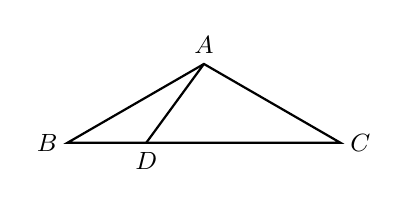
\begin{tikzpicture}[>=stealth, semithick, font=\small, scale=1.0]
  \coordinate (B) at (0,0);
  \coordinate (C) at (3.464,0);
  \coordinate (A) at (1.732,1.0);
  \coordinate (D) at (1.0,0);
  \draw[thick] (A)--(B)--(C)--cycle;
  \draw[thick] (A)--(D);
  \node[above] at (A) {$A$};
  \node[left] at (B) {$B$};
  \node[right] at (C) {$C$};
  \node[below] at (D) {$D$};
\end{tikzpicture}
